\documentclass[10pt,letterpaper]{article}

\usepackage[utf8]{inputenc}
\usepackage[T1]{fontenc}
\usepackage[spanish]{babel}
\usepackage[margin=1.8cm]{geometry}
\usepackage{booktabs}
\usepackage{array}
\usepackage{graphicx}
\usepackage{float}
\usepackage{hyperref}
\usepackage{enumitem}

\setlength{\parskip}{0.35em}
\setlength{\parindent}{0pt}
\setlist[itemize]{leftmargin=1.1em,itemsep=0.1em,topsep=0.1em}

\title{\vspace{-1.2cm}
\normalsize Pontificia Universidad Católica de Chile\\
\normalsize IIC3633 Sistemas Recomendadores\\
\normalsize Marzo--Julio 2026\\[0.35em]
\Large Hito 1: Propuesta, Análisis y Baselines\\
\large Recomendación musical personalizada a partir de historiales de escucha de Last.fm}
\author{Agustin Llambias \and Amaya Quero \and Larry Uribe}
\date{}

\begin{document}
\maketitle
\vspace{-0.8cm}

\section{Descripción del problema y justificación}

Los servicios de música digital concentran catálogos muy grandes, por lo que un usuario puede tener dificultades para descubrir canciones o artistas alineados con sus gustos. En este contexto, un sistema recomendador permite ordenar el catálogo y sugerir ítems relevantes usando información histórica de interacciones. El proyecto se enfoca en recomendación musical personalizada usando registros de escucha como retroalimentación implícita: si un usuario escuchó una canción, se asume una señal positiva de interés, aunque no exista una calificación explícita.

El problema principal es: dado el historial de escucha de un usuario, recomendar canciones o artistas que el usuario no haya escuchado previamente y que tengan alta probabilidad de ser relevantes para él. Este caso es representativo de sistemas recomendadores reales porque trabaja con feedback implícito, alta cardinalidad de ítems, sesgos de popularidad y posibles cambios temporales en las preferencias.

El dataset utilizado es \textit{Last.FM\_dataset} de Kaggle, disponible en \url{https://www.kaggle.com/datasets/harshal19t/lastfm-dataset}. En la versión descargada se observan 166.153 registros de escucha, donde cada registro indica usuario, artista, canción, álbum, fecha y hora. Dado que no existen ratings explícitos, cada escucha se interpreta como feedback implícito positivo.

\section{Objetivos del proyecto}

El objetivo general es construir y evaluar un sistema de recomendación musical personalizada sobre datos de Last.fm, comparando baselines simples con métodos más expresivos bajo un protocolo reproducible de evaluación offline.

Los objetivos específicos son:
\begin{itemize}
    \item Caracterizar el dataset mediante análisis descriptivo de usuarios, artistas, canciones, álbumes e interacciones.
    \item Definir un protocolo de train/test para evaluar recomendación top-N con datos implícitos.
    \item Implementar al menos tres modelos de referencia: Random, Most Popular y un modelo específico al dominio musical.
    \item Comparar los modelos usando métricas de ranking como HitRate@10, Precision@10, MAP@10 y nDCG@10.
    \item Desarrollar en Midterm un método más avanzado, como filtrado colaborativo item-item, factorización matricial para feedback implícito o un enfoque híbrido.
\end{itemize}

\section{Análisis descriptivo de los datos}

Se define cada ítem como el par artista-canción, con el fin de distinguir canciones con el mismo nombre interpretadas por artistas distintos. La Tabla~\ref{tab:dataset} resume las estadísticas principales del dataset.

\begin{table}[h]
\centering
\small
\begin{tabular}{lrlr}
\toprule
\textbf{Métrica} & \textbf{Valor} & \textbf{Métrica} & \textbf{Valor}\\
\midrule
Registros & 166.153 & Usuarios & 11\\
Artistas & 22.823 & Ítems artista-canción & 76.038\\
Tracks por nombre & 67.241 & Álbumes & 38.629\\
Duplicados exactos & 0 & Álbumes faltantes & 12\\
Rango temporal & \multicolumn{3}{l}{01-01-2021 a 31-01-2021}\\
Sparsity usuario-ítem & \multicolumn{3}{l}{0,8411}\\
\bottomrule
\end{tabular}
\caption{Resumen descriptivo del dataset Last.fm descargado desde Kaggle.}
\label{tab:dataset}
\end{table}

La matriz usuario-ítem tiene densidad aproximada de 15,89\%. Aunque este valor no es extremadamente disperso, el catálogo sigue siendo amplio en relación con el número de usuarios. La distribución de interacciones por usuario es desbalanceada: el usuario con menos registros tiene 1.063 escuchas, mientras que el máximo alcanza 33.695. A nivel de ítems existe una cola larga: la mayoría de canciones aparece una o dos veces, mientras que unos pocos ítems concentran muchas escuchas.

Los artistas más escuchados incluyen Sophie, Madlib, Bicep, Taylor Swift y Arlo Parks. Entre los ítems más frecuentes aparecen \textit{Metric - Cascades (Dirt Road Version)} y \textit{Ocean Waves For Sleep - Rolling Ocean Waves}. Estos patrones justifican incluir un baseline de popularidad y, al mismo tiempo, evaluar métodos personalizados que no se limiten a recomendar solamente los ítems globalmente dominantes.

\begin{figure}[H]
    \centering
    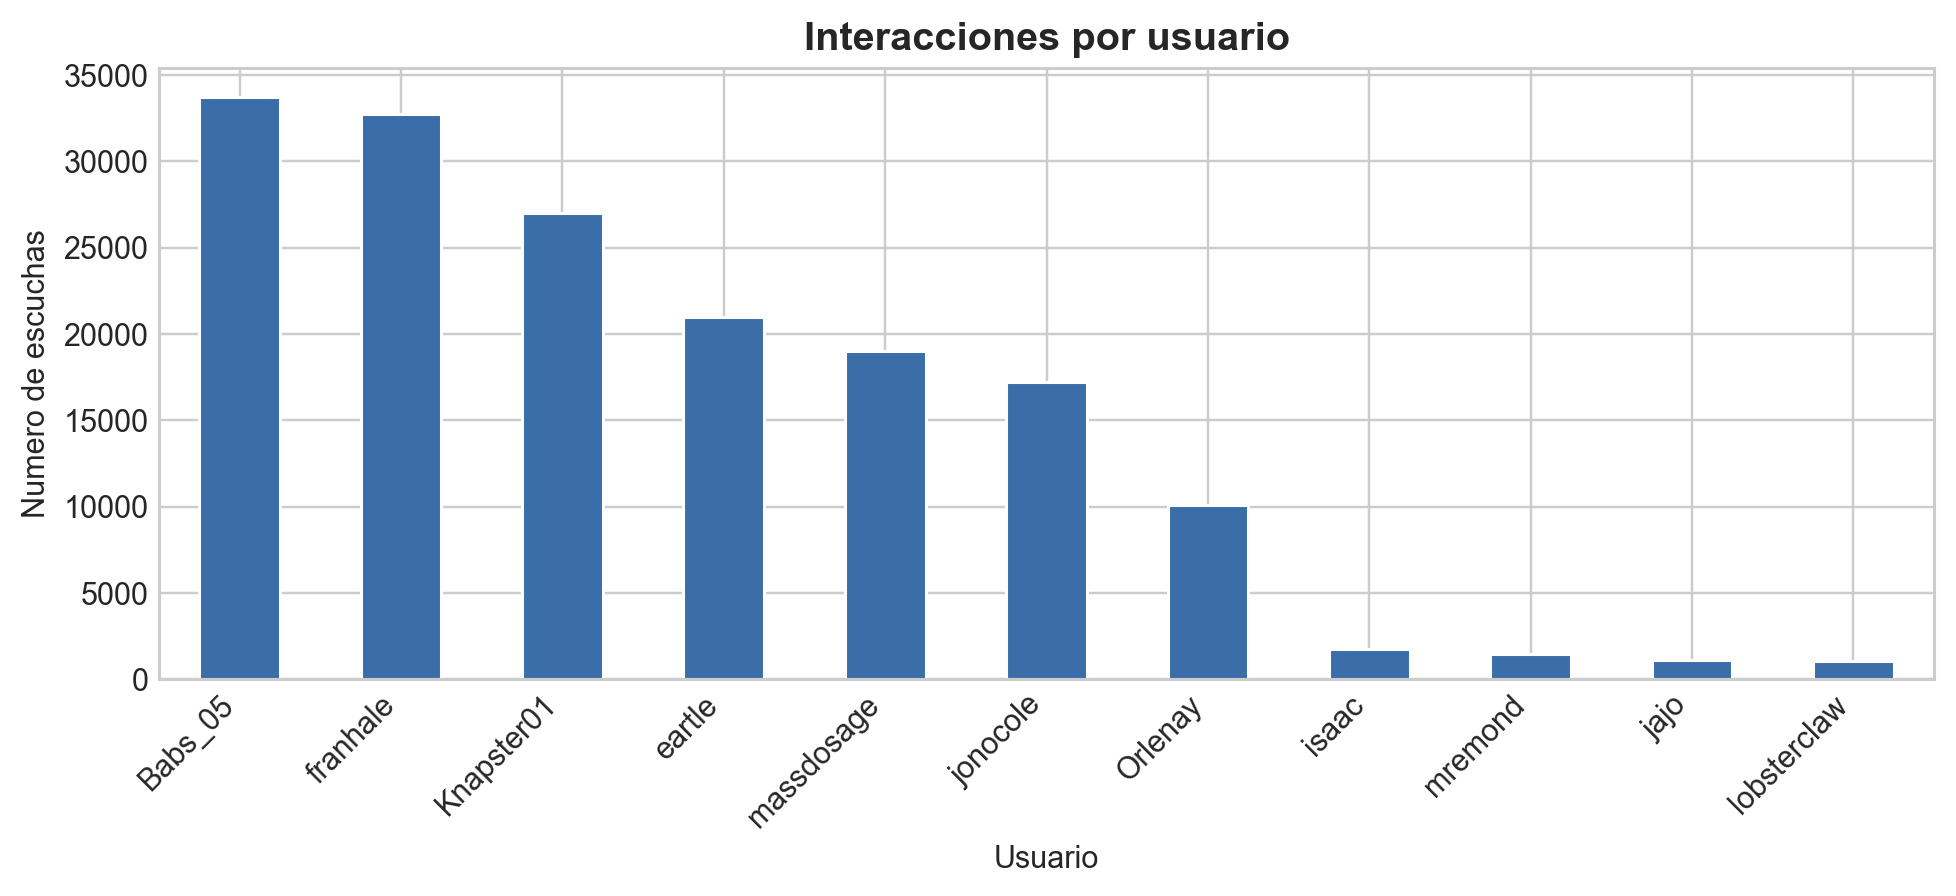
\includegraphics[width=0.48\textwidth]{figures/interacciones_por_usuario.png}
    \hfill
    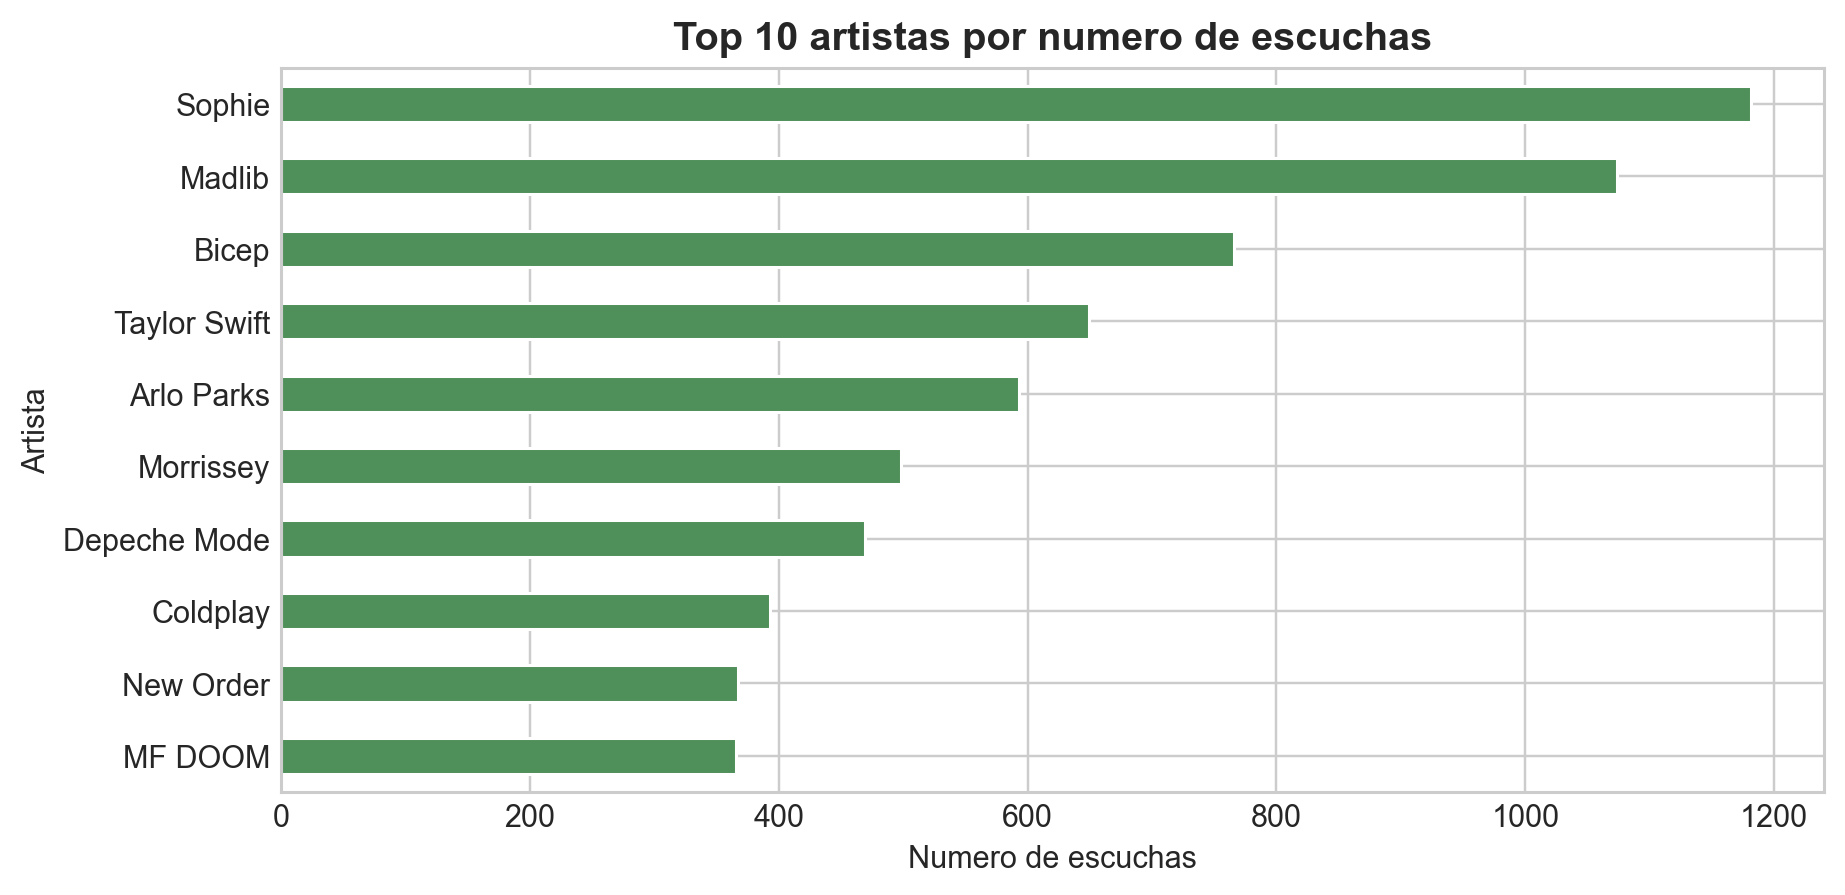
\includegraphics[width=0.48\textwidth]{figures/top_artistas.png}
    \caption{Distribución de escuchas por usuario y artistas más frecuentes en el dataset.}
    \label{fig:eda-usuarios-artistas}
\end{figure}

\begin{figure}[H]
    \centering
    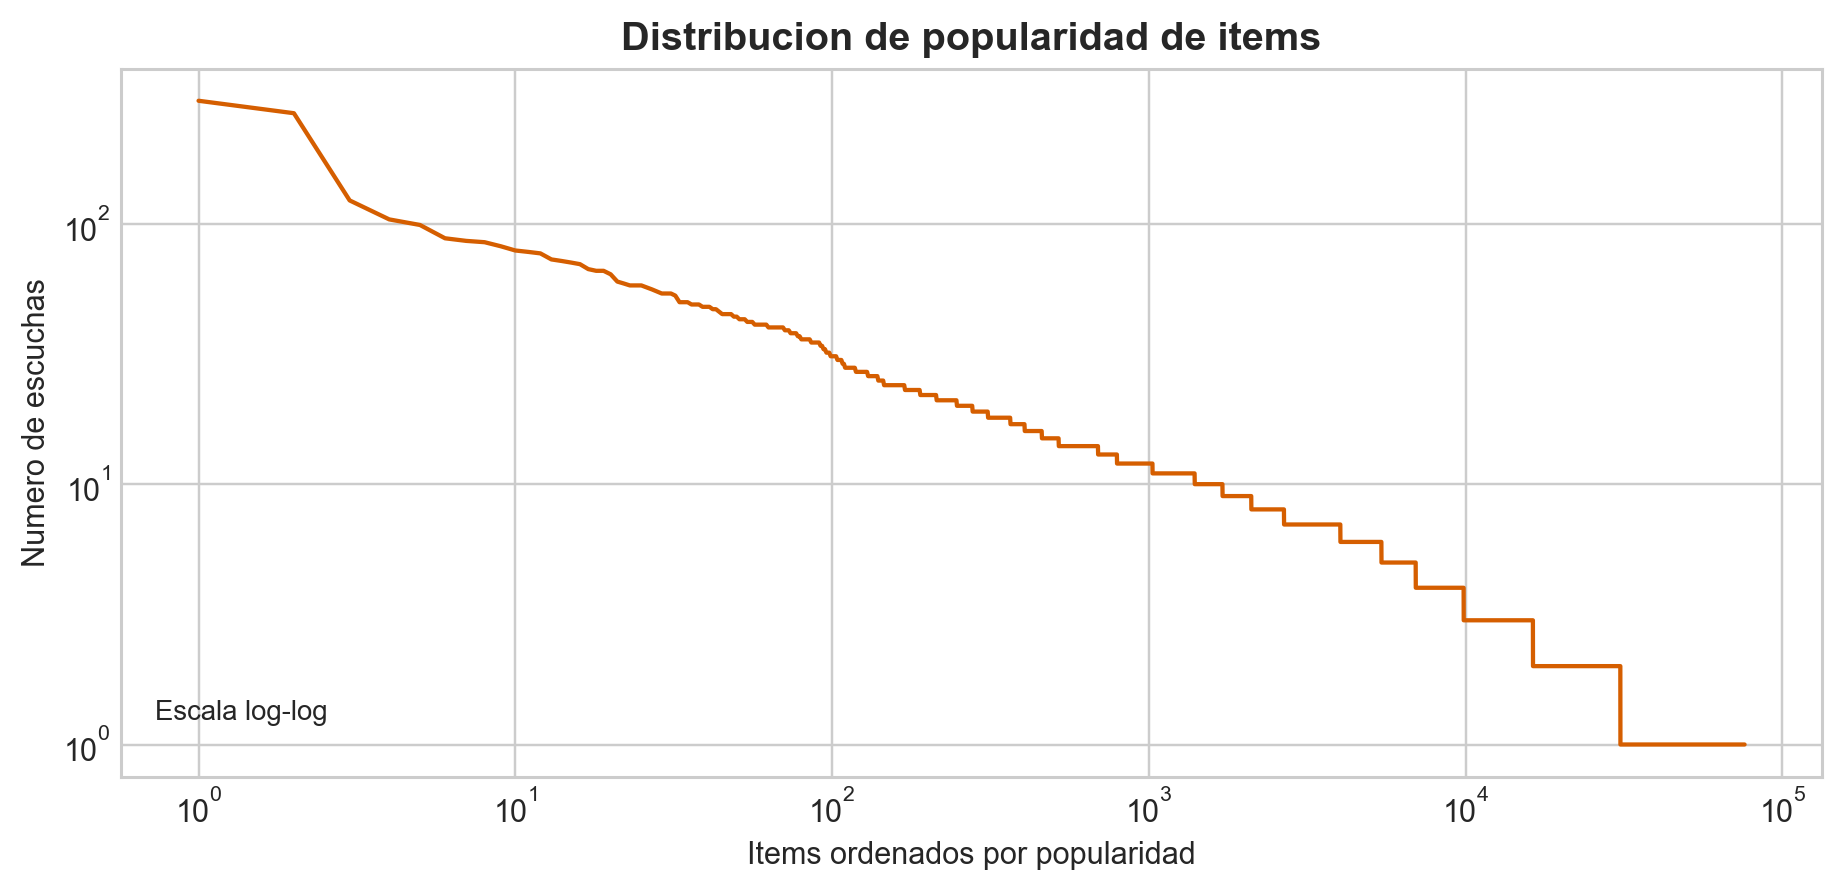
\includegraphics[width=0.72\textwidth]{figures/distribucion_popularidad_items.png}
    \caption{Distribución de popularidad de ítems en escala log-log. La forma de cola larga muestra que pocos ítems concentran muchas escuchas, mientras que la mayoría aparece pocas veces.}
    \label{fig:long-tail}
\end{figure}

\section{Baselines y protocolo experimental}

La evaluación usa split temporal por usuario: el 80\% inicial de sus escuchas queda en train y el 20\% final en test. Los ítems relevantes son canciones futuras que el usuario no había escuchado en train. Esta decisión evita filtración de información futura hacia el entrenamiento y se ajusta mejor a un escenario real de recomendación musical que un split aleatorio.

Se implementaron tres modelos de referencia:
\begin{itemize}
    \item \textbf{Random:} recomienda canciones aleatorias no vistas por el usuario. Sirve como control mínimo para verificar el protocolo.
    \item \textbf{Most Popular:} recomienda las canciones más frecuentes en train. No es personalizado, pero captura el sesgo global de popularidad.
    \item \textbf{Favorite Artist Popular:} identifica los artistas más escuchados por cada usuario en train y recomienda canciones populares de esos artistas que el usuario aún no haya escuchado.
\end{itemize}

Las métricas utilizadas son HitRate@10, Precision@10, MAP@10 y nDCG@10. HitRate@10 mide si existe al menos un acierto en el top 10; Precision@10 mide la proporción de recomendaciones relevantes; MAP@10 considera la posición de los aciertos; y nDCG@10 premia que los ítems relevantes aparezcan más arriba en el ranking.

\begin{table}[h]
\centering
\small
\begin{tabular}{lrrrr}
\toprule
\textbf{Modelo} & \textbf{HitRate@10} & \textbf{Precision@10} & \textbf{MAP@10} & \textbf{nDCG@10}\\
\midrule
Random & 0,3636 & 0,0364 & 0,0074 & 0,0310\\
Most Popular & 0,0909 & 0,0455 & 0,0202 & 0,0367\\
Favorite Artist Popular & 0,4545 & 0,0455 & 0,0133 & 0,0459\\
\bottomrule
\end{tabular}
\caption{Resultados preliminares de baselines con split temporal por usuario.}
\label{tab:resultados}
\end{table}

El baseline personalizado por artista obtiene el mayor HitRate@10 y nDCG@10, lo que sugiere que la afinidad histórica usuario-artista aporta una señal personalizada útil. Most Popular logra el mejor MAP@10, mostrando que la popularidad global sigue siendo competitiva para ordenar algunos aciertos tempranos.

Estos resultados deben interpretarse con cautela. Random obtiene un HitRate@10 relativamente alto porque cada usuario conserva, en promedio, 2.291 ítems relevantes futuros bajo el split temporal. Por lo tanto, HitRate@10 es poco exigente en este primer experimento y debe complementarse con Precision@10, MAP@10 y nDCG@10. Para Midterm se propone evaluar también con negative sampling o con un test set más restringido por usuario.

El código que respalda la carga de datos, el análisis descriptivo, las figuras y los baselines se encuentra en el notebook \texttt{Hito\_1\_LastFM.ipynb} y en el script reproducible \texttt{hito1\_lastfm\_baselines.py}.

\begin{figure}[H]
    \centering
    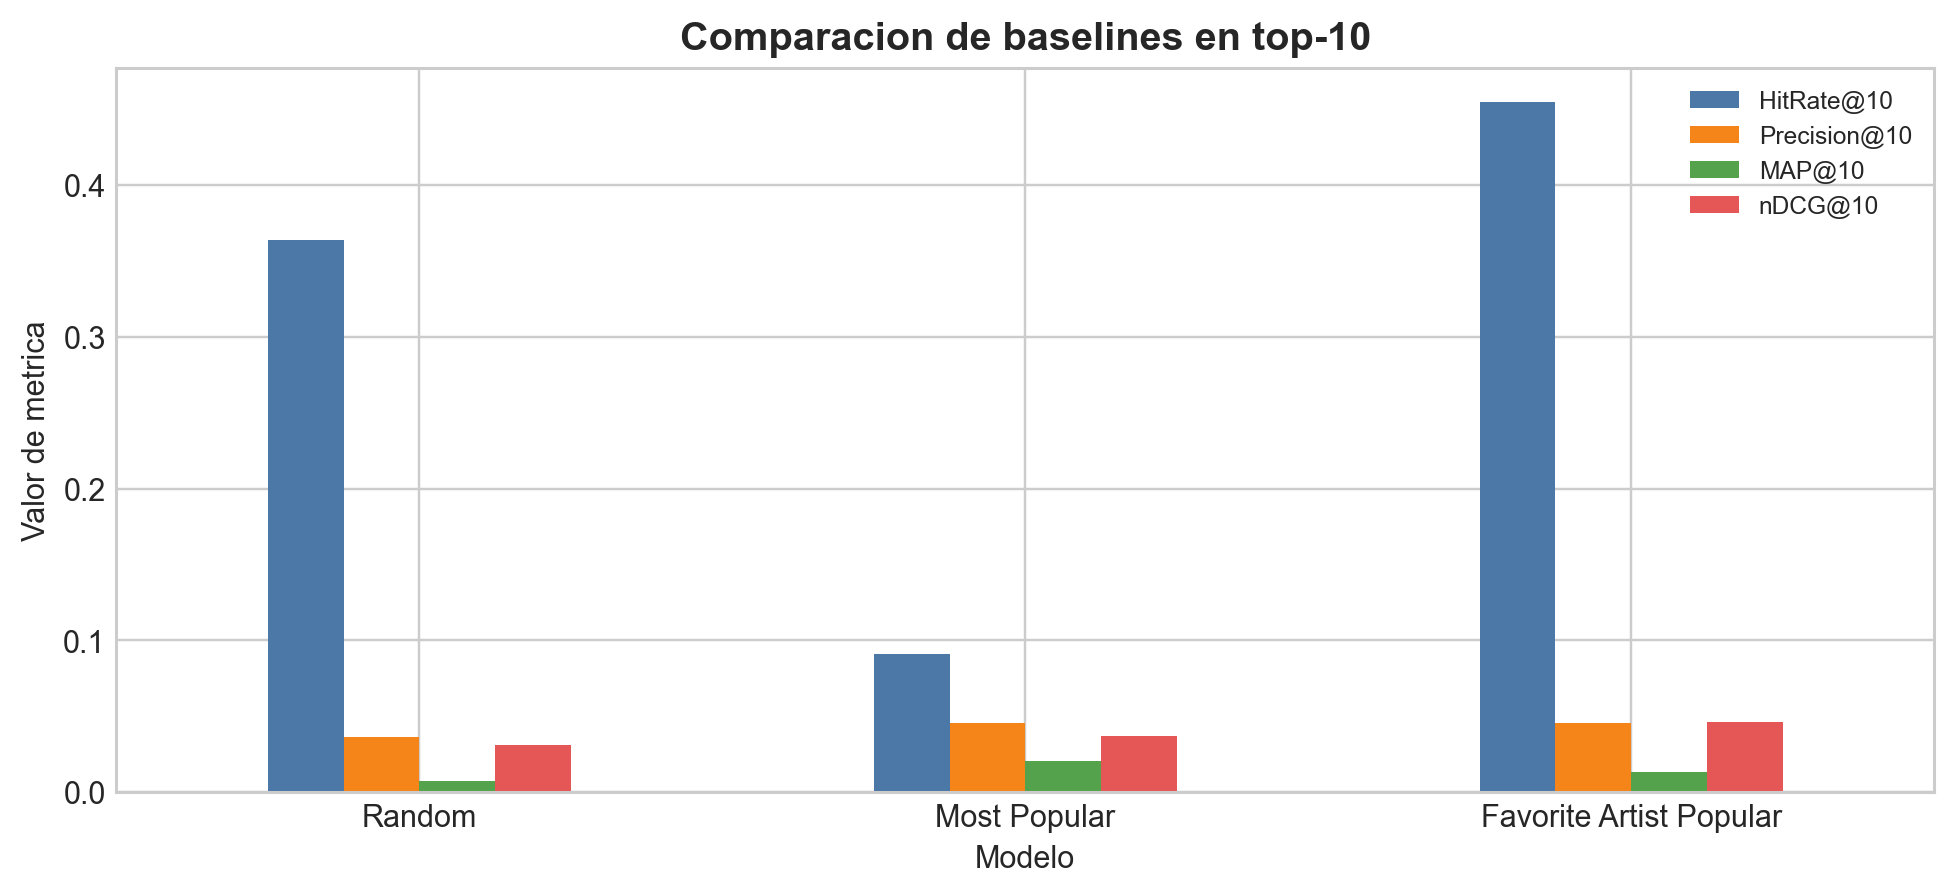
\includegraphics[width=0.82\textwidth]{figures/metricas_baselines.png}
    \caption{Comparación visual de las métricas top-10 para los tres baselines implementados.}
    \label{fig:metricas-baselines}
\end{figure}

\section{Planificación para Midterm}

\begin{table}[h]
\centering
\small
\begin{tabular}{p{2.3cm}p{4.2cm}p{7.2cm}}
\toprule
\textbf{Fecha} & \textbf{Actividad} & \textbf{Resultado esperado}\\
\midrule
08/05 & Cierre Hito 1 & Propuesta, EDA y baselines iniciales documentados.\\
09/05--16/05 & Limpieza y normalización & Pipeline reproducible y matriz usuario-ítem.\\
17/05--24/05 & Filtrado colaborativo & Modelos user-user e item-item con distintas similitudes.\\
25/05--31/05 & Método avanzado & Factorización matricial para feedback implícito o método híbrido.\\
01/06--04/06 & Evaluación y análisis & Tabla comparativa, análisis de errores y limitaciones.\\
05/06 & Entrega Midterm & Informe intermedio con resultados preliminares.\\
\bottomrule
\end{tabular}
\caption{Plan de trabajo propuesto para el Hito 2.}
\label{tab:plan}
\end{table}

Los criterios de éxito para Midterm serán superar Most Popular en al menos una métrica de ranking top-K, mantener cobertura razonable de usuarios e ítems, reportar tiempos de ejecución y dejar el pipeline documentado para reproducir resultados.

\section{Limitaciones y riesgos}

La principal limitación del dataset descargado es el bajo número de usuarios: existen solo 11 usuarios, aunque cada uno tiene muchas interacciones. Esto permite estudiar personalización a nivel individual, pero limita la generalización estadística de resultados agregados. Para mitigar este problema, en Midterm se reportarán métricas por usuario y se analizará la sensibilidad al protocolo de evaluación.

Otra limitación es que el dataset no incluye ratings explícitos ni información semántica rica como géneros o tags. Para este hito se trabajó con feedback implícito y metadatos básicos. En la siguiente etapa se evaluará si conviene enriquecer el dataset o concentrarse en métodos colaborativos que exploten mejor la matriz de escuchas.

\section{Bibliografía}

\begin{itemize}
    \item Harshalsps19t. \textit{Last.FM\_dataset}. Kaggle, 2023. \url{https://www.kaggle.com/datasets/harshal19t/lastfm-dataset}
    \item Sgardelis, K., Margaris, D., Spiliotopoulos, D. y Vassilakis, C. \textit{An evaluation review of user similarity metrics in sparse collaborative filtering datasets}. International Journal of Data Science and Analytics, 2025.
    \item Koren, Y., Bell, R. y Volinsky, C. \textit{Matrix factorization techniques for recommender systems}. Computer, 42(8), 30--37, 2009.
    \item He, X., Deng, K., Wang, X., Li, Y., Zhang, Y. y Wang, M. \textit{LightGCN: Simplifying and Powering Graph Convolution Network for Recommendation}. SIGIR, 2020.
\end{itemize}

\end{document}
